\section{State-of-the-art classification methods}

\subsection{Classification methods}
	In this project, the following classification methods are used to classify the data:

	\subsubsection*{Support Vector Machine (SVM)}
		The Support Vector Machine (SVM) constitutes a supervised learning approach accompanied by learning algorithms designed to examine data for both classification and regression analysis purposes. When provided with a collection of training instances, each labeled as part of either of two distinct categories, an SVM training algorithm constructs a model capable of categorizing new instances into either of these two categories. In essence, it functions as a non-probabilistic binary linear classifier\cite{suthaharan2016support}.
	
	\subsubsection*{Random Forest (RFC)}
		Random forests, also known as random decision forests, stand as an ensemble learning technique employed for tasks encompassing classification, regression, and other similar objectives. This method functions by generating numerous decision trees during the training phase and subsequently determining the class that appears most frequently among these trees for classification tasks, or calculating the average prediction for regression tasks. Notably, at its core, it employs decision trees as fundamental classifiers.\cite{belgiu2016random}. 
	
	\subsubsection*{K-Nearest Neighbors (k-NN)}
		The k-nearest neighbors algorithm is a method in pattern recognition for classification and regression. It operates by assessing the k closest training examples in the feature space. For classification, it assigns an object to the most common class among its k nearest neighbors via majority vote. In regression, it calculates an output based on the average prediction of these neighbors.\cite{kramer2013k}.

	\subsubsection*{Gaussian Naive Bayes (GNB)}
		Naive Bayes classifiers in machine learning use Bayes' theorem with simple feature independence assumptions. They're basic Bayesian models and can handle continuous data with Kernel Density Estimation. With good pre-processing, it compete with more advanced methods including support vector machines. It also finds application in automatic medical diagnosis\cite{perez2006supervised}.
	
	\subsubsection*{Decision Tree Classifier (DTC)}
		Decision tree learning employs a decision tree as a predictive model to deduce conclusions about an item's target value based on observations. This technique finds use in statistics, data mining, and machine learning. When dealing with a discrete set of target values, it's termed a classification tree. In this setup, leaves indicate class labels, and branches represent feature combinations leading to these labels. When the target values are continuous, as in real numbers, it's referred to as a regression tree.\cite{navada2011overview}.
	
	\subsubsection*{Linear Discriminant Analysis (LDA)}
		Linear discriminant analysis, also known as normal discriminant analysis (NDA) or discriminant function analysis, extends Fisher's linear discriminant. This technique is employed in statistics, pattern recognition, and machine learning to determine a linear combination of features that distinguishes or separates multiple classes of objects or events. The resulting combination can function as a linear classifier or, more commonly, aid in reducing dimensionality before subsequent classification.\cite{izenman2013linear}.

\subsection{Evaluation methods}
	The evaluation methods used in this project are:
	\subsubsection{Cross-validation}
		Cross-validation is a method of evaluating machine learning (ML) models by training multiple ML models on subsets of the available input data and evaluating them on the remaining subset\cite{browne2000cross}. In k-fold cross-validation, the input data is split into $k$ subsets of data (also known as folds). Then iterate over each fold, training a model on the $k-1$ remaining folds and evaluating it on the fold left out. The performance measure reported by k-fold cross-validation is an average of the values calculated in the loop. This approach is resource intensive, but it is often more efficient than generating all possible training/test partitions\cite{browne2000cross}.

		Cross-validation is performed using the \emph{Stratified K-Fold} technique to evaluate the performance of each classifier. Metrics such as \emph{accuracy}, \emph{precision}, \emph{recall} and \emph{F1-score} are calculated and recorded. The results are aggregated and displayed in tabular form, providing insights into the initial accuracy and performance of each classifier. The results are also visualized using a bar chart to provide a more intuitive comparison between the classifiers.

	\subsubsection{Confusion matrix}
		Confusion matrix is a table used to describe the performance of a classifier on a set of test data for which the true values are known. The confusion matrix itself is simple to understand, but the related terminology can be confusing. The terms \emph{positive (TP \& FP)} and \emph{negative (TN \& FN)} refer to the classifier's prediction, and the terms \emph{true} and \emph{false} refer to whether that prediction corresponds to the external judgment. In this project, the confusion matrix is used to visualize the performance of each classifier. The confusion matrix is also used to calculate the \emph{accuracy}, \emph{precision}, \emph{recall} and \emph{F1-score} of each classifier\cite{townsend1971theoretical}.

		Confusion matrices are generated to visualize the classification performance of each refined classifier. Heatmap of the correlation matrix for the original features are also created to show correlations among features. Refer to \appendixname~\ref{appdx:confusionMatrixOfAllTheSixClassifiers} for the confusion matrix heatmap. 

\subsection{Evaluation process}
	The evaluation is performed in three phases, State-of-the-art (Raw), dimensionality reduction and hyperparameter optimization to determine the effect of feature selection and hyperparameter optimization on the performance of each classifier. To avoid external factors such as multithreading and CPU usage, the execution was performed 99 times and recorded all the results. The average of the results is used to determine the performance of each classifier. Detail results can be found \href{https://github.com/AkshayChikhalkar/GPU-Classification/tree/main/Text%20Reports}{here}\footnote{https://github.com/AkshayChikhalkar/GPU-Classification/tree/main/Text\%20Reports}.
	For visualization, due to wide range of values, the logarithmic scale is used to plot the results. The results are also normalized to provide a more intuitive performance comparison between the classifiers in different phases.

	The results were benchmarked on a system with the following specifications: Apple MacBook Air 13" (2021) with Apple M1 chip, 16GB RAM and 256GB SSD, macOS Sonoma beta 14.0 (23A5328b), Python 3.9.13, scikit-learn 0.24.2, NumPy 1.21.1, Pandas 1.3.1, Matplotlib 3.4.2, Seaborn 0.11.1, Jupyter Notebook 6.4.0, Visual Studio Code 1.81.1. Python was not natively optimized for Apple M1 silicon and was running through the x86 translation layer (emulator) Rosetta 2, for further details about the execution information refer to \appendixname~\ref{appdx:executionDetails}. The execution time might have been affected by the number of threads used (Total threads = 31), considering the multithreading handling of modern SOCs.

\subsubsection{Performance evaluation}
	Performance evaluation of state-of-the-art classification methods is performed using the evaluation methods described above. For Cross-validation, the data is split into 10 folds. The results are aggregated and displayed in tabular form, providing insights into the initial accuracy and performance of each classifier \tablename~\ref{tab:performance_before}. The results are also visualized using a bar chart to provide a more intuitive comparison between the classifiers \figurename~\ref{fig:performance_before_plot}. Here are the performance of each classifier before dimensionality reduction and hyperparameter optimization:

	\begin{figure}[H]
		\centering
		\begin{subfigure}{0.45\textwidth}
			\centering
			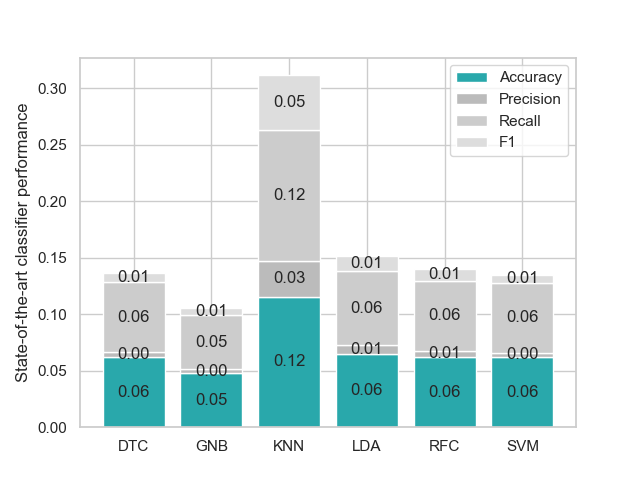
\includegraphics[width=\textwidth]{Plots/Performance_before.png}
			\caption{Visualization}
			\label{fig:performance_before_plot}
		\end{subfigure}%
		\begin{subfigure}{0.55\textwidth}
			\centering
			\small
			\begin{tabular}{|c|c|c|c|c|c|c|c|}
				\hline
					\textbf{Algorithm} &\textbf{Accuracy} &\textbf{Precision} &\textbf{Recall} &\textbf{F1} &\textbf{E.T. (Sec)} \\ \hline
					\hline
					DTC    & 0.062   & 0.004   & 0.062  & 0.008   & 0.001 \\ \hline
					GNB    & 0.048   & 0.003   & 0.048  & 0.006   & 0.001 \\ \hline
					KNN    & 0.115   & 0.032   & 0.115  & 0.049   & 0.007 \\ \hline
					LDA    & 0.065   & 0.008   & 0.065  & 0.013   & 0.001 \\ \hline
					RFC    & 0.062   & 0.006   & 0.062  & 0.011   & 0.007 \\ \hline
					SVM    & 0.062   & 0.004   & 0.062  & 0.007   & 0.057 \\				
				\hline
			\end{tabular}
			\caption{Averaged results of 99 runs}
			\label{tab:performance_before}
		\end{subfigure}
		\caption{Classifier performance before optimization}
	\end{figure}